\documentclass{article}
% The file ijcai11.sty is the style file for IJCAI-11 (same as ijcai07.sty).
\usepackage{ijcai11}

% Use the postscript times font!
\usepackage{times}
\usepackage[utf8x]{inputenc}
\usepackage{datetime}
\usepackage{graphicx}
\usepackage{dblfloatfix}
%\usepackage{stfloats}
\usepackage{mathptmx}
\usepackage[T1]{fontenc}

% the following package is optional:
\usepackage{latexsym}

% Following comment is from ijcai97-submit.tex:
% The preparation of these files was supported by Schlumberger Palo Alto
% Research, AT\&T Bell Laboratories, and Morgan Kaufmann Publishers.
% Shirley Jowell, of Morgan Kaufmann Publishers, and Peter F.
% Patel-Schneider, of AT\&T Bell Laboratories collaborated on their
% preparation.

% These instructions can be modified and used in other conferences as long
% as credit to the authors and supporting agencies is retained, this notice
% is not changed, and further modification or reuse is not restricted.
% Neither Shirley Jowell nor Peter F. Patel-Schneider can be listed as
% contacts for providing assistance without their prior permission.

% To use for other conferences, change references to files and the
% conference appropriate and use other authors, contacts, publishers, and
% organizations.
% Also change the deadline and address for returning papers and the length and
% page charge instructions.
% Put where the files are available in the appropriate places.


\title{Master 1 MoSIG Research Project Report\\
Learning Job Runtimes in Homogenous HPC Systems}
\author{Valentin Reis\\
Supervised by: Denis Trystram \& Eric Gaussier.\\
}

\begin{document}

\maketitle

{% Mosig student
  {\hbox to0pt{\vbox{\baselineskip=10dd\hrule\hbox
to\hsize{\vrule\kern3pt\vbox{\kern3pt
\hbox{{\small I understand what plagiarism entails and I declare that this report }}
\hbox{{\small is my own, original work. }}
\hbox{{\small Name, date and signature: }}
\kern3pt
}\hfil%\kern3pt
\vrule
}\hrule}
}}
}


\begin{abstract}
  Lorem ipsum dolor sit amet, consetetur sadipscing elitr, sed diam nonumy eirmod
  tempor invidunt ut labore et dolore magna aliquyam erat, sed diam voluptua. At
  vero eos et accusam et justo duo dolores et ea rebum. Stet clita kasd gubergren,
  no sea takimata sanctus est Lorem ipsum dolor sit amet.
\end{abstract}

\section{Introduction}
High Performance Computing (HPC) systems are complex machinery at the frontier between research in scheduling and systems engineering. We outline two of the main difficulties that resource management software in this field have to face.

First, the ephemeral nature, and broad range of existing architectures of those systems make the development and application of theoretical results difficult.
New schemes for distributing resources are more present than ever. Many recent systems have complex network and memory/hard drive sharing topologies. Moreover, the topology of HPC systems can now change on a hourly to monthly basis, since the hardware of distributed systems can be reconfigured or extended continually.
Finding scheduling and resource management strategies which can deal with complex systems and adapt to their evolutions poses a challenge.

In addition, the data (i.e.\ the characteristics of the tasks to be executed) these systems have to work with presents many peculiarities.
The nature of the information which users of the system provide is very often loose (e.g.\ with only upper and/or lower bounds on numerical quantities provided).
For instance, and this will be the focus of this paper, the run time of a given job on a specific system is seldom known in advance, but many cluster management software ask the users for an upper bound on this quantity.

As a consequence of these difficulties most free, open-source and commercial resource management software use simple heuristics that can provide bounds on their performance and/or guarantee a few functional properties.
An example of such a heuristic is the First Come First Serve (FCFS) policy to schedule parallel jobs on a homogenous cluster of machines, which starts jobs as soon as possible, in the exact order they were submitted.
Among other properties (such as robustness to lack of information about the amount of time jobs will run on the system), this strategy guarantees the avoidance of starvation.

\subsection{Research Direction}
The general direction we are headed in with this research project is to deal with the input data of the resource management systems.
Accomodating for this data seems separable enough from the actual scheduling problems for work towards this objective to be rewarding.
No innovative ways to query the data from the users will be studied, we will rely on existing logs from HPC systems. Instead, we seek to apply Machine Learning techniques in order to reduce uncertainty of, and extract information and/or structure from, the input data of the HPC systems.
We will be working with the problem of presenting input data in the most valuable way possible to a scheduling algorithm. How to use this data to the fullest will not be discussed.
When assessing the relevance of the specific information we choose to produce from the job characteristics, references from the scheduling litterature and existing systems will provide ground to stand on.

\subsection{Job runtimes}
Most HPC resource management software (including the SLURM, OpenPBS, OpenLava and OAR software) do ask information about jobs to users, such as topological requests in terms of processing units and memory, the name of the executable, miscellaneous functional requirements and, last but not least, the expected run time of the job with respect to its hardware requirements.
This user-provided estimate of the run time of a job on a specific system will be referred as \textbf{reqtime} in the rest of the paper. Most of these software use the \textbf{reqtime} of a job as an upper bound on its run time, and kill it should \textbf{reqtime} be violated. As a consequence, users overestimate this value, should they choose or be forced to provide it. The following section will present a statistical analysis pertaining to this relationship.

The true run time of a job with respect to a given affected topology is of great interest, as the scheduling policies are highly dependent on this information to provide good solutions \~ref{truc}. We will refer to this quantity as the \textbf{runtime} of a job.
It must be clear that in the context of topological heterogeneity, the \textbf{runtime} of a job is only defined with respect to a specific processing environment to which it might be affected.
This can include, and is not limited to, the network topology of the processing units, the availability of shared memory, message passing costs, and the operating system supporting the computations.

\subsection{Problem Statement}
In this paper, the broad question of refining the data is reduced to a single variable, the \textbf{runtime}. The problem statement we are dealing with is the following.

Given a specific homogenous HPC Cluster with negligible communication costs, how to best predict the value of the \textbf{runtime} of a job?

The choice of dealing with homogenous distributed machines without communication costs in a first approach has the interesting property of separing the data treatment from the scheduling and interaction with the system.
In this case, the \textbf{runtime} becomes an intrinsic attribute of a job.
On the contrary to the input data which is always subject to peculiarities of the various systems and software, the \textbf{runtime} is always present as a simple field in workload logs of HPC systems, such as those available at the workload archive [ref to feitelson].

This problem statement implies a latent question: How to communicate the prediction to the rest of the system (e.g.\ single-value, probability density, confidence factor)? Alternatives will be discussed but ultimately, the focus will be on single-valued predictions.
As mentionned previously, our approach is to use machine learning techniques. We will be inferring runtime from the the job characteristics by learning from system logs, and since this is a value in $[0,+\infty ]$, this is a standard supervised learning problem, namely regression.

We will be careful to only learn our models on logs from homogenous systems, or homogenous subsets of systems which are sizeable enough to learn from.
As for downplaying the impact of communication costs, we will further restrict our work to machines which do not possess overly complex topology or distribute computing nodes across more than a handful of routers.
In essence, we are targeting large Beowulf clusters, supercomputers, GPU farms and mainframe clusters.

\section{Motivation}

\subsection{Importance of \textbf{runtime}}
\label{sub:importance_of_runtime}
Once again, we emphasise the role of the \textbf{runtime} in scheduling tasks. Classical results from scheduling theory use the `clairvoyant' model[ref], where all \textbf{runtimes} of jobs with respect to any affectation on the system being modeled are known.
Informally, if we want to make use of this extensive theoretical body, we must at least reduce uncertainty in this information.
More recent models [ref Trystram FCFS] do [\ldots].
Another approach [ref prob.backfilling] uses predicted probability distributions on the runtimes of jobs in order to take scheduling decisions.
In all cases, reducing uncertainty in \textbf{runtime} is critical to the success of the approach used to schedule jobs.

As mentioned before, existing solutions use much simpler heuristics. We will now focus on a particular system, and outline the reasons why, in the absence of a predictive technique applied the input data, the FCFS heuristic is applied.
% subsection importance_of_runtime (end)

\subsection{Reqtime vs Runtime on a real system}
\label{sub:reqtime_vs_runtime_on_a_real_system}
The following study is conducted on a log[ref log] containing 20 months worth of data from the Curie[ref curie] supercomputer operated by the French government-funded research organization CEA (Commissariat à l'Énergie Atomique). It contains more than 300,000 jobs, submitted from February 2011 to October 2012 by 900 users in the `cleaned' version from the workload archive [ref archive]. The log has several homogenous CPU partitions and CPU+GPU partitions, however in a each partition, all nodes are identical. Jobs are allocated to partitions using user preference. The system is managed using the SLURM (Simple Linux Utility for Resource Management) software.
Figure [ref figure] shows the marginal distributions of \textbf{reqtimes} and \textbf{runtimes} on this system.

\begin{figure*}[b]
  \centering\rule{0.8*\textwidth}{0.3*\textwidth}

        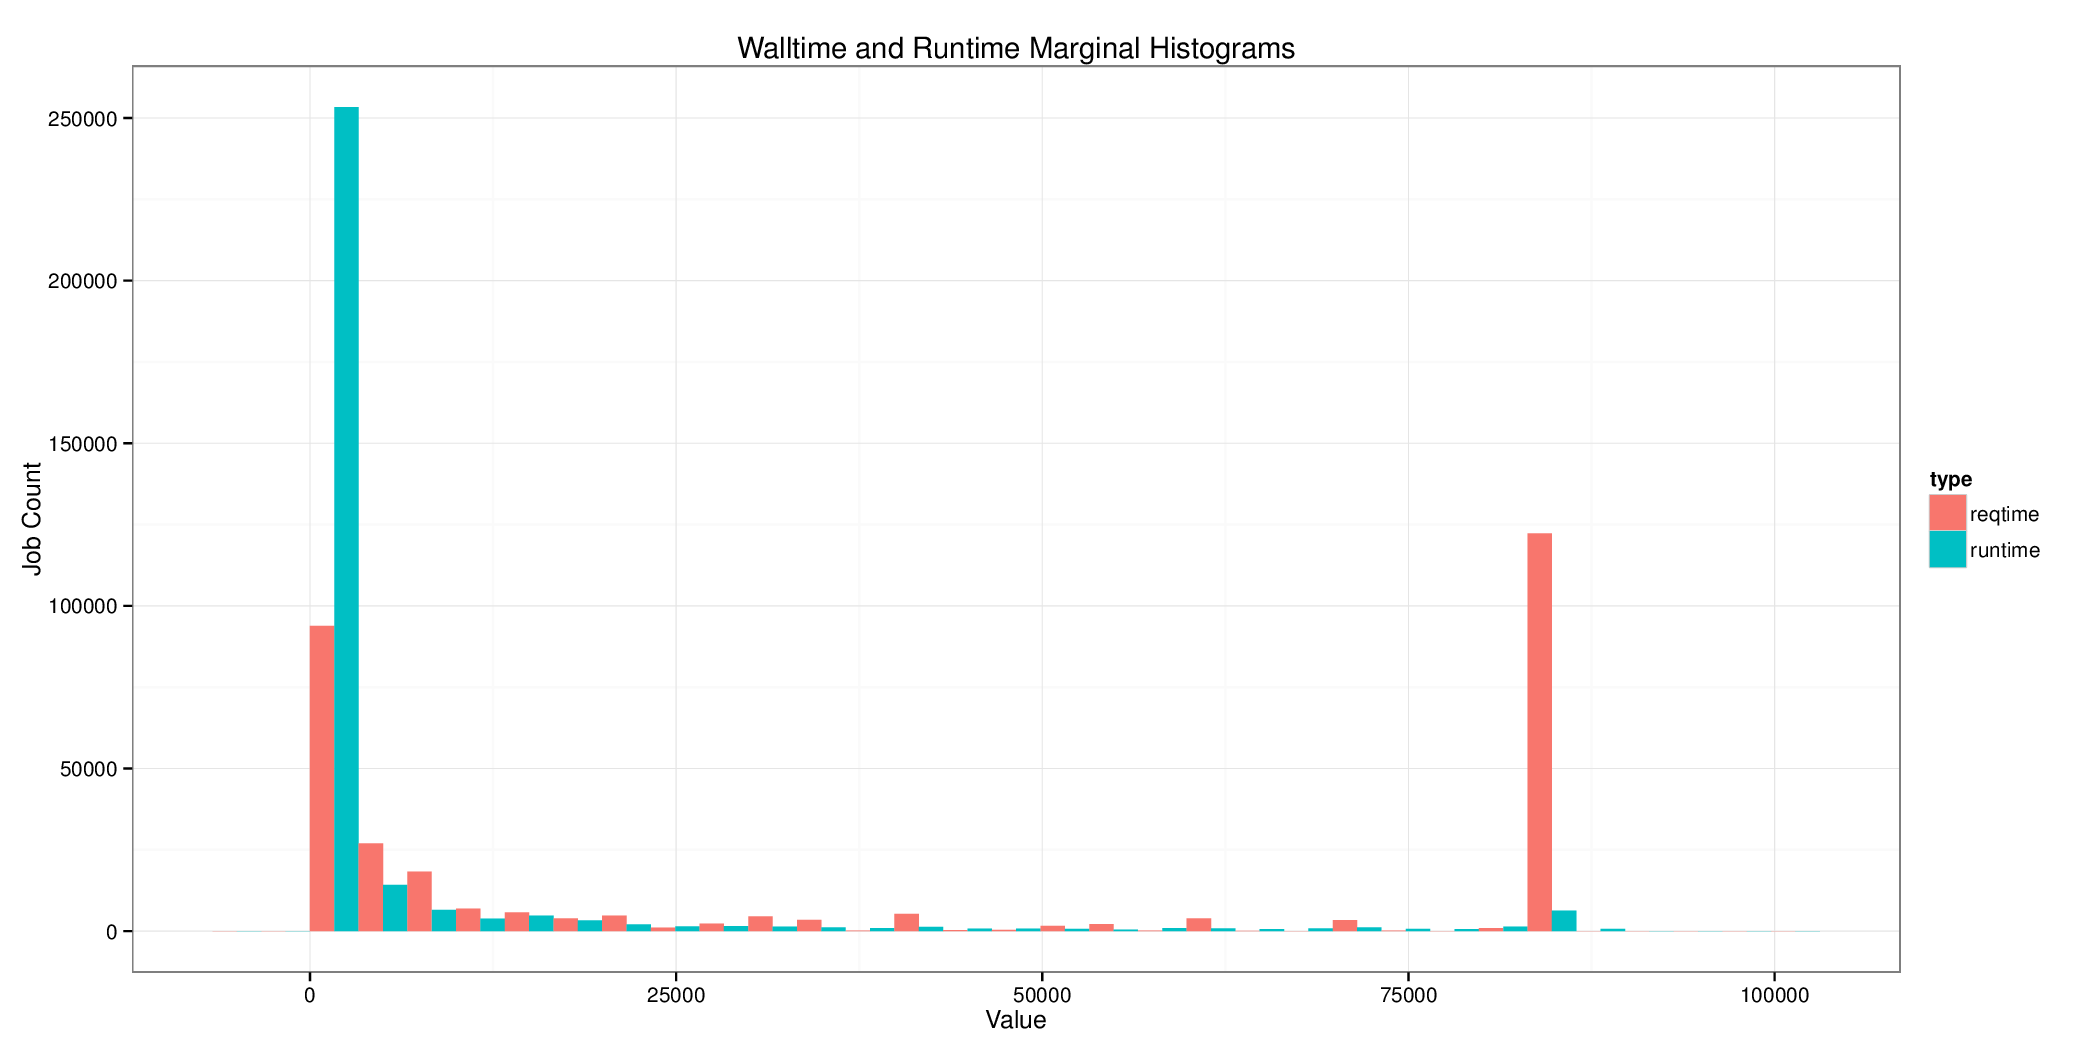
\includegraphics[width=\textwidth]{../../wallimage-0.png}
        \caption{Marginal Histograms of \textbf{reqtime} and \textbf{runtime} of jobs on the CEA Curie log.}
\label{fig:_wall_run_for_report_pdf}
\end{figure*}





TODO: show the curie log.

% subsection reqtime_vs_runtime_on_a_real_system (end)


\section{State of the art in \textbf{runtime} prediction}


\subsection{Nature of the prediction}
\label{sub:nature_of_the_prediction}

TODO: -what to predict: value?, confidence interval?, distribution? whith which algorithms can we use those?

% subsection nature_of_the_prediction (end)

\subsection{Predicting a value}
\label{sub:predicting_a_value}

TODO: -give the references and explain the historical methods, gibbons historical scheduler, the tsafir et al paper with mean of two last runtimes values userwise..

% subsection predicting_a_value (end)

\subsection{Predicting a distribution}
\label{sub:predicting_a_distribution}

TODO: -give the references and explain the probabilistic backfilling thing..

% subsection predicting_a_distribution (end)


\section{Our approach}
\label{sec:our_approach}
WHY ML? well, there is simple little patterns everywhere
\subsection{Random Forests}
\label{sub:random_forests}
TODO: -explain our approach, why it could lead to better results (external info+signal locality(ref hmm thesis for locality..))
% subsection random_forests (end)

\subsection{Explainability}
\label{sub:explainability}
TODO: -explain one advantage of random forests: discussion about the trees after learning..
% subsection explainability (end)

% section our_approach (end)

\section{Preliminary Results}
\label{sec:preliminary_results}

TODO:results..

% section preliminary_results (end)

\section{Conclusions}
\label{sec:conclusions}

TODO:conclure..

% section conclusions (end)


\section{Acknowledgements}
\label{sec:conclusions}

TODO:remercier..

% section conclusions (end)


%% The file named.bst is a bibliography style file for BibTeX 0.99c
\bibliographystyle{named}
\bibliography{report}

\end{document}
